
\chapter{Description de l'API de \PpFf}
\label{description.chap}

\gt{Pour \'eviter la confusion, tu dois utiliser les m\^emes termes
que dans l'API, m\^eme si ces termes sont en anglais. Mais tu les mets
dans la police courrier, avec texttt.}

\begin{figure}[ht]
\centering
     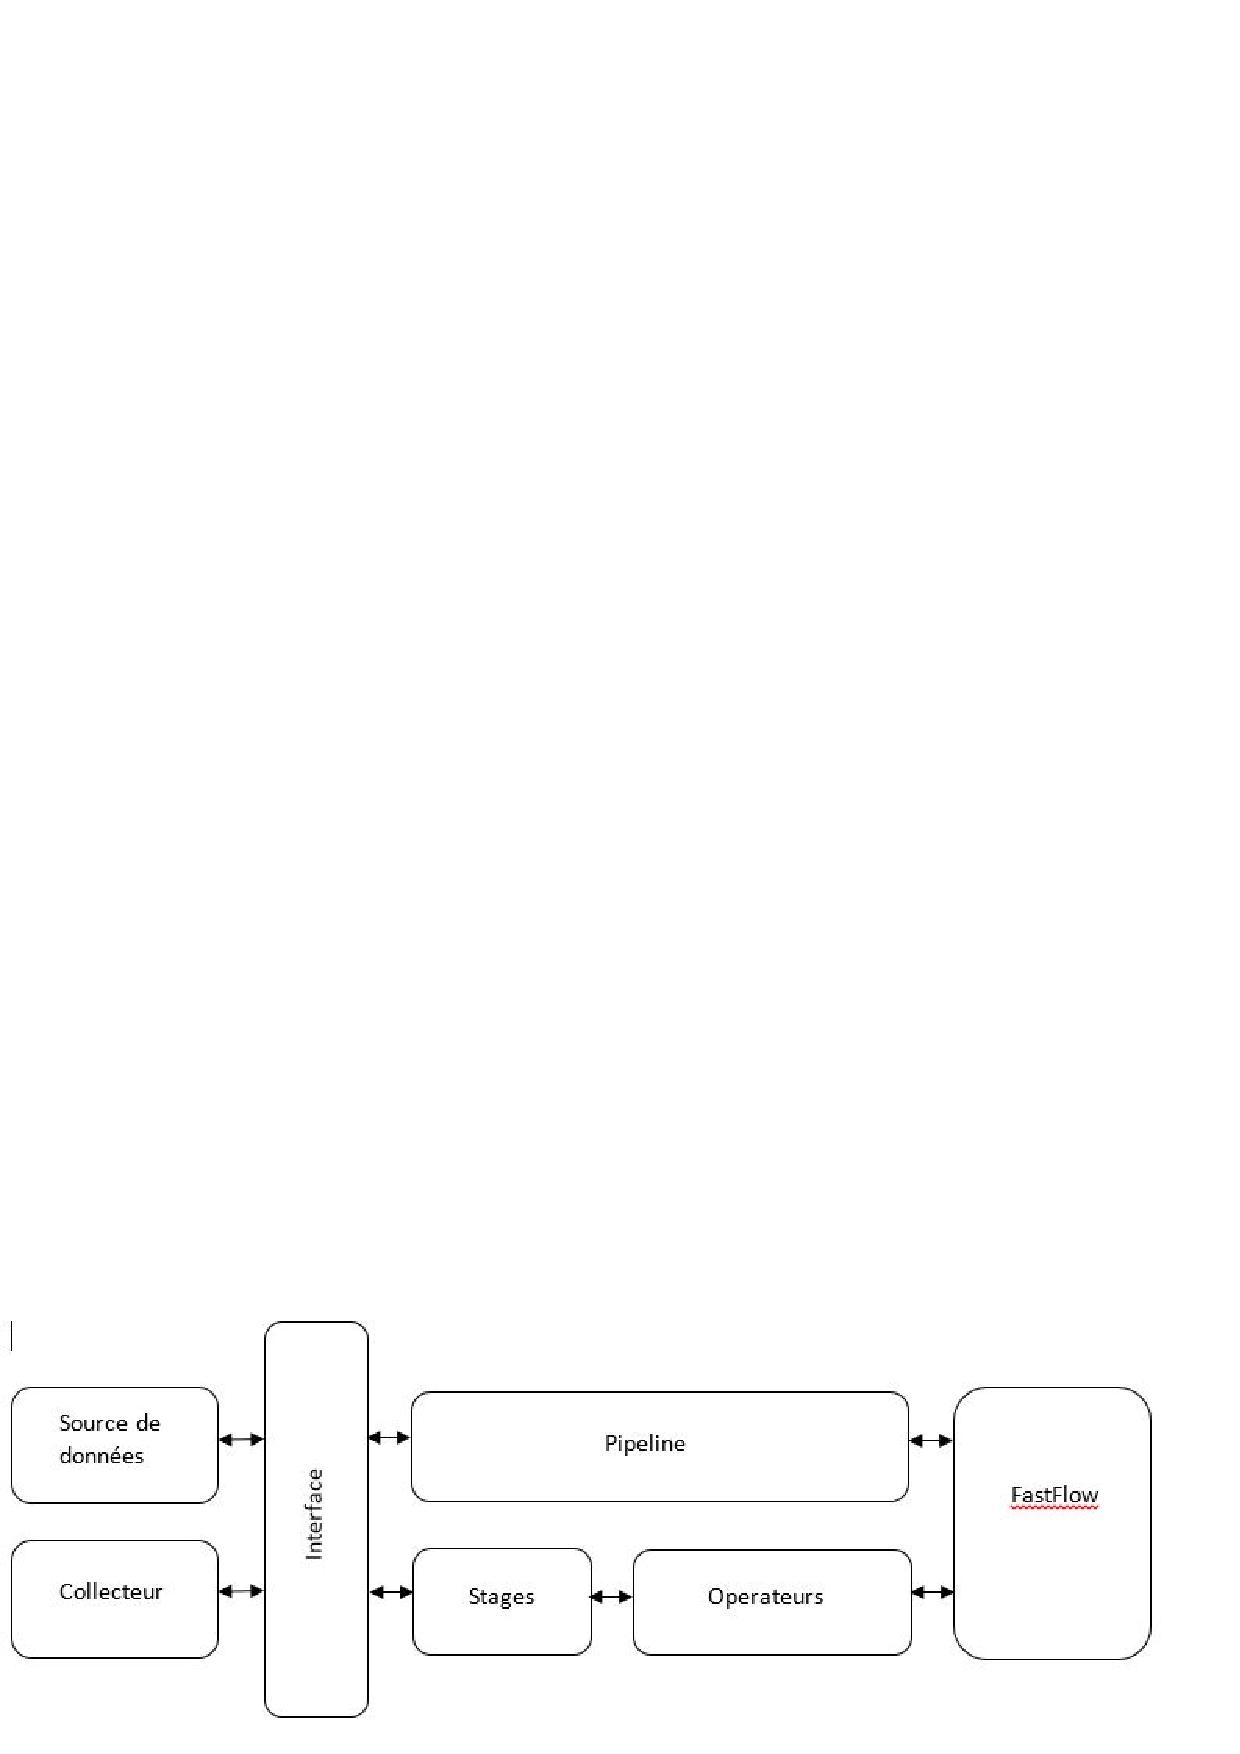
\includegraphics[width=1.0\textwidth]{Figures/ComponentsAPI.jpg}
      \caption{Les composants de l'API de \ppff.}
       \label{ComponentsAPI.fig}
\end{figure}


\GT{Pour ce premier diagramme de classes: il ne faudrait mettre que
les classes qui sont visibles aux utilisateurs, donc les <<concepts>>
qui sont utiles pour utiliser l'API et \^etre capable de s'en
servir. Les autres classes de plus bas niveau (en lien avec FastFlow
par exemple), pourront \^etre pr\'esent\'ees dans le prochain
chapitre.}


Ce chapitre pr\'esente l'API de \ppff. Sa conception permet aux utilisateurs de tirer parti de la simplicit\'e d'utilisation tout en cachant la complexit\'e concernant les m\'ecanismes concurrents utilis\'es. La figure~\ref{ComponentsAPI.fig} pr\'esente une vue d'ensemble de l'architecture de \ppff. L'API est compos\'ee de quatre \'el\'ements principaux: l'Interface avec laquelle le d\'eveloppeur interagit, les \texttt{Pipeline}s --- qui sont le coeur de l'API ---, les \texttt{Stage}s et les \texttt{Operator}s. Le r\^ole de chaque composant dans l'API est pr\'esent\'e dans la section suivante. La derni\`ere section  d\'ecrit plus en d\'etail les principales m\'ethodes de l'interface.



L'\texttt{API} de \texttt{PpFf} est impl\'ement\'e au-dessus de la biblioth\`eque \texttt{FastFlow}, impl\'ementation qui sera d\'ecrite au prochain chapitre.

Le pr\'esent chapitre d\'ecrit le r\^ole de chaque composant de
\texttt{PpFf}. La figure~\ref{fig:ClassDiagramme} pr\'esente une vue
d'ensemble des classes qui composent l'\texttt{API}.

\GT{<<et leur mappage aux mod\`eles de \texttt{FastFlow}>>: Non, dans
le prochain chapitre, pas dans celui-ci!}

%
%\GT{Probablement qu'un diagramme de classe UML serait int\'eressant et
%utile.  Il pourrait \^etre introduit ici, puis expliqu\'e dans les
%sous-sections qui suivent.}
%
%\GT{Note que de fa\c{c}on g\'en\'erale, lorsqu'on d\'ebute une section
%qui contient plusieurs sous-sections, il est pr\'ef\'erable d'avoir
%quelques lignes d'introduction, qui donnent une vue d'ensemble de ce
%qui suit. Pas toujours, mais ici, avec le diagramme de classes, \c{c}a
%ferait l'affaire.}
%
%\IC{Mon plan initial \'etait de d\'ecrire les composants dans le chapitre 2 (Description de l'API de PpFf) et de pr\'esenter la partie technique dans le chapitre 3 (Impl\'ementation). Dans la premi\`ere partie du chapitre 2 j'ai choisi de d\'ecrire les composants principaux de l'API et dans la deuxi\`eme partie de ce chapitre de pr\'esenter quelques m\'ethodes avec des exemples. 
%Dans le chapitre 3 j'ai eu l'intention d'introduire un diagramme de classe UML en expliquant les classes qui compose l'API. } 
%
%\IC{Qu'est-ce que vous en pensez ? Est-ce que je dois introduire le diagramme dans le chapitre 2 ? Je ne suis pas sûr que je fasse la différence entre la description et implémentation de l’API.
%}


%\GT{La description est tout ce qu'un programmeur doit savoir/connaitre
%pour \underline{utiliser} ton API --- de l'ext\'erieur, comme une
%boite noire. L'impl\'ementation d\'ecrit les <<d\'etails>>
%n\'ecessaires pour comprendre \underline{comment fonctionne} l'API,
%par exemple, ce qu'un mainteneur devrait comprendre/connaitre s'il
%voulait modifier, corriger ou \'etendre ton API.}
%
%\GT{En lien avec le diagramme de classes, si l'utilisateur de l'API
%utilise ou manipule diff\'erents concepts et classes dans son
%programme, que ces concepts/classes sont utiles pour pouvoir utiliser
%correctement l'API --- avec la bonne syntaxe et la bonne s\'emantique
%--- alors ces concepts devraient \^etre d\'ecrits, par un diagramme de
%classes par exemple.}

\section{Interface}

\begin{figure}[ht]
\centering
     \includegraphics[width=1.0\textwidth]{Figures/ClassDiagramme.jpg}
      \caption{Les classes qui composent l'\texttt{API}.}
       \label{ClassDiagramme.fig}
\end{figure}


L'interface propos\'ee en PpFf consiste en un ensemble de m\'ethodes qui permettent \`a l'utilisateur de manipuler des flux de donn\'ees de mani\`ere simple et efficace. L'interface suit d'assez pr\`es celle introduite pour les \emph{Streams} de Java~8. Le tableau~\ref{methodes_api.tab} d\'ecrit bri\`evement les m\'ethodes impl\'ement\'ees dans l'API.




%\GT{Dans un tabular, pour mettre du texte, on utilise p avec une
%largeur. Ceci \'evite de mettre des sauts de lignes explicites, ce qui
%n'est jamais une bonne id\'ee.}

%\GT{Il faut mettre le code avec police tt. Par contre, j'ai essay\'e
%que le code soit mis par d\'efaut ainsi, mais cela n'a pas
%fonctionn\'e, d'o\`u les commandes tt ins\'er\'ees en d\'ebut de
%chaque ligne~:(}
%
%\GT{Par contre, le d\'efaut avec la solution actuelle, c'est que c'est
%tr\`es difficile \`a comprendre pour les m\'ethodes plus complexes. Il
%faudra qu'on r\'efl\'echisse \`a une fa\c{c}on plus claire de
%pr\'esenter la signaure des m\'ethodes.}
%
%\IC{J'ai ajout\'e toutes les m\'ethodes d\'efinies dans l'interface de l'API dans ce tableau et j'ai \'et\'e oblig\'e d'utiliser le paquet longtable parce qu'elle s'\'etendait sur plusieurs pages. J'ai essay\'e de pr\'esenter la signature des m\'ethodes dans un format plus concis. Par exemple le paramètre std ::fonction a \'et\'e remplac\'e pour Func; j'ai enlev\'e les mots typename de chaque d\'eclaration de template; le param\`etre <typename ELEM, class ALLOC = std ::allocator<ELEM class TContainer >> a \'et\'e remplac\'e pour Container. De plus je n'ai pas pu r\'eutiliser la fonction qui redimensionne le tableau resizebox(textwidth). J'ai utilis\'e une police de caract\`ere plus petite (tiny) pour pouvoir encadrer le tableau dans la page.
%}
%
%\IC{J'ai reformul\'e la description pour le r\'esultat de la fonction flatMap}


%\begin{landscape}
\newpage
\KOMAoptions{paper=landscape,pagesize}
\recalctypearea


\begin{center}
\footnotesize
\begin{longtable}{|l|l|p{5cm}|}
\caption{Les m\'ethodes publiques de l'API de~\ppff.\label{methodes_api.tab}}\\
\hline
\textbf{M\'ethode} & \textbf{Type du r\'esultat} & \textbf{Description du r\'esultat}\\
\hline
\endfirsthead
\multicolumn{3}{c}%
{\tablename\ \thetable\ Méthodes publiques de l'API (\textit{suite})} \\
\hline
\textbf{M\'ethode} & \textbf{Type du r\'esultat} & \textbf{Description du r\'esultat}\\
\hline
\endhead
\hline \multicolumn{3}{r}{\textit{Suite page suivante}} \\
\endfoot
\hline
\endlastfoot
\hline
	\begin{tabular}{@{}l@{}}
	\tt template<T> \\
	\tt allMatch(Func<bool(T*)> predicate)
	\end{tabular} &
  	\texttt{bool} &
    Retourne \texttt{true} si tous les \'el\'ements
    du flux satisfont \texttt{predicate}, sinon \texttt{false}.
    \\
\hline
	\begin{tabular}{@{}l@{}}
	\tt template<T> \\
	\tt anyMatch(Func<bool(T*)> predicate)
	\end{tabular} &
  	\texttt{bool} & 
    Retourne \texttt{true} si au moins un  
    \'el\'ement du flux satisfait \texttt{predicate}, sinon \texttt{false}.
\\
\hline
	\begin{tabular}{@{}l@{}}
	\tt template<T, Container<T>{>}\\
	\tt collect()
	\end{tabular} &
  	\texttt{Container<T>} &
    Retourne un conteneur
    STL avec tous les \'el\'ements du flux.
    \\
\hline
	\begin{tabular}{@{}l@{}}
	\tt count()\\
	\end{tabular} &
  	\texttt{unsigned int} & 
    Retourne le nombre d'\'el\'ements
    du flux.
    \\
\hline
	\begin{tabular}{@{}l@{}}
	\tt template<In> \\
	\tt find(Func<bool(In*)> const\& predicate)
	\end{tabular} &
  	\texttt{Pipe\&} &
    Retourne les
    \'el\'ements du flux qui satisfont \texttt{predicate}.
    \\
\hline
	\begin{tabular}{@{}l@{}}
	\tt template<In, Out, Container> \\
	\tt flatMap(Func<Container*(In*)> const\& taskFunc)
	\end{tabular} &
  	\texttt{Pipe\&} & 
    Applique la fonction fournie en argument
    \`a chaque \'el\'ement du flux et concat\`ene ces \'el\'ements lorsque plusieurs sont produits par la fonction.
    \\
\hline
	\begin{tabular}{@{}l@{}}
	\tt template<In, Out, Container=In> \\
	\tt flatMap()
	\end{tabular} &
  	\texttt{Pipe\&} &
    Produit un flux avec les \'el\'ements du conteneur.  
    \\
\hline
	\begin{tabular}{@{}l@{}}
	\tt template<In, K=In, V=In, MapType> \\
	\tt groupByKey(Func<K*(In*)> fk, Func<V*(In*)> fv)
	\end{tabular} &
  	\texttt{MapType} &
    Retourne un dictionnaire (\emph{map}) avec les \'el\'ements
    du flux regroupés par cl\'e.
   \\
\hline
%	\begin{tabular}{@{}l@{}}
%	\tt template<T, Container> \\
%	\tt intermediateCollect()
%	\end{tabular} &
%	\texttt{Collection<T, Container>} &
%    Retourne une collection avec les
%    \'el\'ements du flux. \GT{Est-ce utile de mentionner cette m\'ethode?}
%    \\ 
%\hline
	\begin{tabular}{@{}l@{}}
	\tt template<T> \\
	\tt limit(int n)
	\end{tabular} &
	\texttt{Pipe\&} & 
    Retourne un flux compos\'e des \texttt{n}~premiers \'el\'ements du flux d'entr\'ee.
    \\
\hline
	\begin{tabular}{@{}l@{}}
	\tt linesFromFile(string\& path)
	\end{tabular} &
	\texttt{Pipe\&} & 
    Retourne un flux avec les lignes
    contenues dans le fichier indiqu\'e par \texttt{path}.
    \\
\hline
	\begin{tabular}{@{}l@{}}
	\tt template<In, Out> \\
	\tt map(Func<Out*(In*)> const\& taskFunc)
	\end{tabular} &
	\texttt{Pipe\&} & 
    Retourne un flux compos\'e de
    l'application de \texttt{taskFunc}
    \`a chacun des
    \'el\'ements du flux.
    \\
\hline
	\begin{tabular}{@{}l@{}}
	\tt template<T> \\
	\tt max(Func<void(T*, T*)> compare)
	\end{tabular} &
	\texttt{T} &
	Retourne l'\'el\'ement maximum du flux en fonction du comparateur.
    \\
\hline
	\begin{tabular}{@{}l@{}}
	\tt template<T> \\
	\tt min(Func<void(T*, T*)> compare)
	\end{tabular} &
	\texttt{T} &
	Retourne l'\'el\'ement minimum du flux en fonction du comparateur.
    \\
\hline
	\begin{tabular}{@{}l@{}}
	\tt template<T> \\
	\tt noneMatch(Func<bool(T*)> predicate)
	\end{tabular} &
	\texttt{bool} &
    Retourne \texttt{true} si aucun des \'el\'ements
    du flux ne satisfait \texttt{predicate},
    sinon \texttt{false}.
    \\
\hline
	\begin{tabular}{@{}l@{}}
	\tt parallel(int workers = 1)
	\end{tabular} &
	\texttt{Pipe\&} &
	Sp\'ecifie le nombre de travailleurs \`a utiliser pour traiter les \'el\'ements du flux.
    \\
\hline
	\begin{tabular}{@{}l@{}}
	\tt template<In> \\
	\tt peek(Func<void(In*)> const\& taskFunc)
	\end{tabular} &
	\texttt{Pipe\&} &
	Applique la fonction \texttt{taskFunc} \`a chaque \'el\'ement du flux et r\'e\'emet l'\'el\'ement (sans le modifier) sur le flux de sortie. Note: Utile pour le d\'ebogage.
    \\
\hline
	\begin{tabular}{@{}l@{}}
	\tt template<In, Out=In> \\
	\tt reduce(Reducer<In, Out> const\& reducer)
	\end{tabular} &
	\texttt{Out} &
	Effectue une r\'eduction sur les \'el\'ements du flux. Voir la notion de \texttt{reducer}, p.~\pageref{reducer.sect}.
    \\
\hline
	\begin{tabular}{@{}l@{}}
	\tt template<In, Out=In> \\
	\tt reduce(Out init, Func<Out(In, Out)> acc)
	\end{tabular} &
	\texttt{Out} &
	Effectue une r\'eduction des \'el\'ements du flux, en utilisant \texttt{init} comme valeur initiale et \texttt{acc} comme fonction d'accumulation.
    \\
\hline
	\begin{tabular}{@{}l@{}}
	\tt template<In, K=In, V=In, MapType> \\
	\tt reduceByKey(Reducer<In, V> r, Func<K*(In*)> fk)
	\end{tabular} &
	\texttt{MapType} &
    Effectue une r\'eduction sur les valeurs de chaque cl\'e à l'aide d'op\'erateur \texttt{Reducer}. Voir la notion de \texttt{Reducer}, p.~\pageref{reducer.sect}.
    \\
\hline
	\begin{tabular}{@{}l@{}}
	\tt template<T> \\
	\tt skip(int n)
	\end{tabular} &
	\texttt{Pipe\&} &
    Retourne un flux compos\'e des \'el\'ements du flux d'entr\'ee, mais en omettant les \texttt{n} premiers \'el\'ements.
    \\
\hline
	\begin{tabular}{@{}l@{}}
	\tt template<T> \\
	\tt sort(Func<bool(T, T)> const\& compare)
	\end{tabular} &
	\texttt{Collection<T, Container>} &
	Effectue le tri des \'el\'ements du flux, selon l'ordre sp\'ecifi\'e par \texttt{compare}. Note: Le premier \'el\'ement du flux de sortie n'est \'emis \emph{qu'apr\`es que la fin de flux ait \'et\'e rencontr\'ee}.
    \\
\hline
	\begin{tabular}{@{}l@{}}
	\tt template<T, Iterator> \\
	\tt source(Iterator  begin, Iterator end)
	\end{tabular} &
	\texttt{Pipe\&} &
	Convertit un conteneur de type \texttt{STL} en flux.
    \\
\hline
	\begin{tabular}{@{}l@{}}
	\tt template<T> \\
	\tt sum()
	\end{tabular} &
	\texttt{T} &
	Retourne la somme des \'el\'ements du flux.
    \\
\hline
\end{longtable}
\normalsize
\end{center}




%\end{landscape}
\newpage
\KOMAoptions{paper=portrait,pagesize}
\recalctypearea







%\begin{table}[h]
%\centering
%
%\resizebox{\textwidth}{!}{%
%
%\begin{tabular}{|l|l|p{8cm}|}
%\hline
%\textbf{M\'ethode} & \textbf{Type du r\'esultat} & \textbf{Description du r\'esultat}\\
%\hline
%	\begin{tabular}{@{}l@{}}
%	\tt template<T> \\
%	\tt allMatch(Func<bool(T*)> predicate)
%	\end{tabular} &
%  	\texttt{bool} &
%    Retourne \texttt{true} si tous les \'el\'ements
%    du flux correspondent au pr\'edicat
%    fourni, sinon \texttt{false}.
%    \\
%\hline
%	\begin{tabular}{@{}l@{}}
%	\tt template<T> \\
%	\tt anyMatch(Func<bool(T*)> predicate)
%	\end{tabular} &
%  	\texttt{bool} & 
%    Retourne \texttt{true} si au moins un  
%    \'el\'ement du flux correspondent
%    au pr\'edicat fourni, sinon \texttt{false}.
%\\
%\hline
%	\begin{tabular}{@{}l@{}}
%	\tt template<T, Container<T>>\\
%	\tt collect()
%	\end{tabular} &
%  	\texttt{Container<T>} &
%    Retourne un conteneur de type
%    STL contenant les \'el\'ements du flux.
%    \\
%\hline
%	\begin{tabular}{@{}l@{}}
%	\tt count()\\
%	\end{tabular} &
%  	\texttt{unsigned int} & 
%    Retourne le nombre d'\'el\'ements
%    dans ce flux.
%    \\
%\hline
%	\begin{tabular}{@{}l@{}}
%	\tt template<In> \\
%	\tt find(Func<bool(In*)> const\& taskFunc)
%	\end{tabular} &
%  	\texttt{Pipe\&} &
%    Retourne tous les
%    \'el\'ements du flux qui satisfont la 
%    fournie en argument.
%    \\
%\hline
%	\begin{tabular}{@{}l@{}}
%	\tt template<In, Out, Container> \\
%	\tt flatMap(Func<Container*(In*)> const\& taskFunc)
%	\end{tabular} &
%  	\texttt{Pipe\&} & 
%    Applique la fonction fournie en argument
%    \`a chaque \'el\'ement du flux.
%    \\
%\hline
%	\begin{tabular}{@{}l@{}}
%	\tt template<In, Out, Container=In> \\
%	\tt flatMap()
%	\end{tabular} &
%  	\texttt{Pipe\&} &
%    \GT{Reformuler: je ne comprends pas la diff\'erence avec le pr\'ec\'edent}    
%    \\
%\hline
%	\begin{tabular}{@{}l@{}}
%	\tt template<In, K=In, V=In, MapType> \\
%	\tt groupByKey(Func<K*(In*)> fk, Func<V*(In*)> fv)
%	\end{tabular} &
%  	\texttt{MapType} &
%    Retourne un dictionnaire (\emph{map}) avec les \'el\'ements
%    du flux regroupés par cl\'e.
%   \\
%\hline
%	\begin{tabular}{@{}l@{}}
%	\tt template<T, Container> \\
%	\tt intermediateCollect()
%	\end{tabular} &
%	\texttt{Collection<T, Container>} &
%    Retourne une collection avec les
%    \'el\'ements du flux.
%    \\ 
%\hline
%	\begin{tabular}{@{}l@{}}
%	\tt template<T> \\
%	\tt limit (int n)
%	\end{tabular} &
%	Pipe\& & 
%    Renvoie dans le flux seulement
%    les n premiers \'el\'ements de
%    ce flux.
%    \\
%\hline
%	\begin{tabular}{@{}l@{}}
%	\tt linesFromFile(string\& path)
%	\end{tabular} &
%	Pipe\& & 
%    Renvoie dans le flux les lignes
%    contenues dans un fichier.
%    \\
%\hline
%	\begin{tabular}{@{}l@{}}
%	\tt template<In, Out> \\
%	\tt map(Func<Out*(In*)> const\& taskFunc)
%	\end{tabular} &
%	Pipe\& &
%    Renvoie dans le flux les
%    r\'esultats constitu\'es de 
%    l'application d'une fonction 
%    fournie en param\`etre aux 
%    \'el\'ements du flux.
%    \\
%\hline
%	\begin{tabular}{@{}l@{}}
%	\tt template<T> \\
%	\tt max(Func<void(T*, T*)> compare)
%	\end{tabular} &
%	\texttt{T} &
%	Retourne l'\'el\'ement maximum du flux en fonction du comparateur fourni en param\`etre.
%    \\
%\hline
%	\begin{tabular}{@{}l@{}}
%	\tt template<T> \\
%	\tt min(Func<void(T*, T*)> compare)
%	\end{tabular} &
%	\texttt{T} &
%	Retourne l'\'el\'ement minimum du flux en fonction du comparateur fourni en param\`etre.
%    \\
%\hline
%	\begin{tabular}{@{}l@{}}
%	\tt template<T> \\
%	\tt noneMatch(Func<bool(T*)> predicate)
%	\end{tabular} &
%	\texttt{bool} &
%	Retourne l'\'el\'ement minimum du flux en fonction du comparateur fourni en param\`etre.
%    \\
%\hline
%	\begin{tabular}{@{}l@{}}
%	\tt parallel(int workers = 1)
%	\end{tabular} &
%	Pipe\& &
%	D\'efinis le nombre de travailleurs fourni en param\`etre.
%    \\
%\hline
%	\begin{tabular}{@{}l@{}}
%	\tt template<In> \\
%	\tt peek(Func<void(In*)> const\& taskFunc)
%	\end{tabular} &
%	Pipe\& &
%	M\'ethode utilis\'ee pour d\'ebogage. Applique une fonction sur les \'el\'ements du flux sans modifier leur valeur.
%    \\
%\hline
%	\begin{tabular}{@{}l@{}}
%	\tt template<In, Out=In> \\
%	\tt reduce(Reducer<In, Out> const\& reducer)
%	\end{tabular} &
%	\texttt{Out} &
%	reduce description.
%    \\
%\hline
%	\begin{tabular}{@{}l@{}}
%	\tt template<In, Out=In> \\
%	\tt reduce(Out init, Func<Out(In, Out)> acc)
%	\end{tabular} &
%	\texttt{Out} &
%	reduce description.
%    \\
%\hline
%	\begin{tabular}{@{}l@{}}
%	\tt template<In, K=In, V=In, MapType> \\
%	\tt reduceByKey(Reducer<In, V> r, Func<K*(In*)> fk)
%	\end{tabular} &
%	\texttt{MapType} &
%	reduceByKey description.
%    \\
%\hline
%	\begin{tabular}{@{}l@{}}
%	\tt template<T> \\
%	\tt skip(int n)
%	\end{tabular} &
%	Pipe\& &
%	skip description.
%    \\
%\hline
%	\begin{tabular}{@{}l@{}}
%	\tt template<T> \\
%	\tt sort(Func<bool(T, T)> const\& compare)
%	\end{tabular} &
%	\texttt{Collection<T, Container>} &
%	sort description.
%    \\
%\hline
%	\begin{tabular}{@{}l@{}}
%	\tt template<T, Iterator> \\
%	\tt source(Iterator  begin, Iterator end)
%	\end{tabular} &
%	Pipe\& &
%	source description.
%    \\
%\hline
%	\begin{tabular}{@{}l@{}}
%	\tt template<T> \\
%	\tt sum()
%	\end{tabular} &
%	\texttt{T} &
%	sum description.
%    \\
%\hline
%
%
%\end{tabular}
%}
%\caption{Les m\'ethodes expos\'ees aux utilisateurs par l'API de \ppff.}
%\label{methodes_api.tab}
%\end{table}




Comme on peut le voir dans le tableau~\ref{methodes_api.tab}, la d\'eclaration des m\'ethodes utilise la programmation g\'en\'erique de C++, c'est-\`a-dire les \emph{templates}. Cela permet aux utilisateurs d'avoir une interface g\'en\'erique unique, de sorte qu'une m\'ethode peut \^etre r\'eutilis\'ee pour n'importe quel type de donn\'ees.


Un autre point cl\'e dans cette interface est son expressivit\'e. M\^eme avant sa conception d\'etaill\'ee, nous nous \'etions donn\'es comme objectif de fournir un syst\`eme suffisamment intuitif et expressif pour le traitement de flux de donn\'ees. 

\gt{Lorsque dans le texte tu indiques des identificateurs qui viennent du code --- find, collect, etc. --- alors il faut les mettre en police tt, donc \texttt{find}, \texttt{collect}, etc.}


\begin{Listing}
{\small
\begin{lstlisting}
// Definition (omise) d'un vecteur d'objets Employe.
std::vector<Employe> sourceEmployes;
...

std::vector<Employe> result = 
   Pipe()
   .source<Employe>(sourceEmployes.begin(), sourceEmployes.end())
   .find<Employe>([](Employe *e) { return e->salary > 35000; })
   .collect<Employe, std::vector>();
\end{lstlisting}
}
\caption{Un exemple illustrant l'\'expressivit\'e de l'API de \ppff.}
\label{expressivite_api.c++}
\end{Listing}

\GT{Voir note plus bas sur position des listings et des references.}

Le listing~\ref{expressivite_api.c++} pr\'esente un extrait de code C++ qui donne un premier aper\c{c}u de l'expressivit\'e de l'interface --- d'autres exemples seront pr\'esent\'es plus loin. Dans cet exemple, on s\'electionne les employ\'es qui ont un salaire plus grand que 35~K\$. Les employ\'es sont initialement dans un conteneur STL et sont filtr\'es en chainant trois op\'erations : $i)$ \texttt{source} qui permet d'envoyer dans le flux des objets de type~\texttt{Employe}; $ii$) \texttt{find} qui s\'electionne les employ\'es selon la condition fournie en param\`etre (une lambda-expression); $iii)$ \texttt{collect} qui met les employ\'es s\'electionn\'es dans un conteneur STL. Ici, les employ\'es s\'electionn\'es sont mis dans un conteneur de type \texttt{std::vector} --- le type de conteneur est donn\'e par le type fourni en argument (g\'en\'erique) de la m\'ethode \texttt{collect}.




\section{Op\'erateurs}

Les op\'erateurs (classe \texttt{Operator}) sont la base de notre syst\`eme. L'API fournit un ensemble d'op\'erateurs qui facilitent la t\^ache de l'utilisateur. Les op\'erateurs sont structur\'es en deux cat\'egories : les op\'erateurs sans \'etat et les op\'erateurs avec \'etat.

Les \emph{op\'erateurs sans \'etat} sont ceux qui ne disposent pas d'informations sur l'it\'eration en cours et ne transmettent pas les informations interm\'ediaires des \'etapes de traitement pr\'ec\'edentes. Si on prend comme exemple le filtre repr\'esent\'e par la m\'ethode \texttt{find} du tableau~\ref{methodes_api.tab}, il traite le flux de donn\'ees \'el\'ement par \'el\'ement. 
%
Lorsque la fonction (lambda-expression) fournie en argument \`a la m\'ethode \texttt{find} ne satisfait pas la condition lorsqu'appliqu\'ee \`a un \'el\'ement du flux, le filtre ne retourne rien. 

Les \emph{op\'erateurs avec \'etat} sont ceux qui maintiennent une structure de donn\'ees interne, qui repr\'esente l'\'etat. Cette structure repr\'esente ou synth\'etise l'historique des \'el\'ements pass\'es au flux et affecte la logique de traitement dans les calculs ult\'erieurs. Par exemple, l'op\'erateur \texttt{Sum} calcule la somme des \'el\'ements du flux. Son \'etat contient la valeur de la somme de tous les \'el\'ements qui pr\'ec\'edent celui en cours de traitement. 

\subsection*{Op\'erateurs de r\'eduction}

\label{reducer.sect}

\begin{Listing}[tbp]
\begin{lstlisting}
 template< typename In, typename Out >
 class Reducer{
       Reducer(Out init, 
               Func<Out(Out, In)> const& accumulator,
               Func<Out(Out, Out)> const& combiner)

       Reducer(Func<Out(Out, In)> const& accumulator,
               Func<Out(Out, Out)> const& combiner)

       Reducer(Out init, 
               Func<Out(Out, In)> const& accumulator)
 }
\end{lstlisting}
\caption{La signature pour l'op\'erateur \texttt{Reducer}.}
\label{reducer.c++}
\end{Listing}

\GT{Une règle utile à savoir pour \LaTeX: lorsqu'on met un élément
flottant (avec caption/label, e.g., figure, table, pseudocode,
listing), il est préférable de mettre cet élément \underline{avant} la
première référence (et non pas après).  La position du flottant par
rapport au texte qui y réfère est alors meilleure.}

\GT{Pour les exemples de code, il est préférable d'utiliser Listing
(définie dans macros.tex) et lstlisting (package \LaTeX) plutot que
alltt --- ce qui évite d'avoir à mettre un backslash devant une
accolade. J'ai configure pour que par defaut ce soit avec le langage
C++ (on peut faire de la coloration syntaxique, mais pas utile dans un
mémoire.  On peut aussi spécifier un autre langage, avec une mise en
forme différente.}

L'op\'erateur de classe \texttt{Reducer} est utilis\'e pour r\'eduire les \'el\'ements du flux \`a une valeur unique. Le listing~\ref{reducer.c++} présente la spécification  de la classe \texttt{Reducer} avec les signatures des fonctions associées. 

Un \texttt{Reducer} est construit avec une valeur initiale, une fonction \texttt{accumulator} et une fonction \texttt{combiner}. La valeur initiale et la fonction \texttt{combiner} sont optionnelles gr\^ace \`a la surcharge du constructeur. Lorsque ces arguments sont omis, la valeur initiale est initialis\'ee \`a la valeur par d\'efaut du type de cette valeur et la fonction \texttt{combiner} est remplac\'ee par la fonction \texttt{accumulator}. La fonction \texttt{combiner} est utilis\'ee lorsque le flux est trait\'e en parall\`ele, par plusieurs \emph{threads}. Dans un tel cas, le flux est divis\'e en sous-flux --- i.e., chaque \emph{thread} traite un sous-ensembles des éléments --- qui sont r\'eduits en parall\`ele avec la fonction \texttt{accumulator}. Les r\'esultats partiels produits par les divers \emph{threads} sont ensuite combin\'es, dans le \emph{thread} principal, avec la fonction \texttt{combiner}. 





\section{Pipeline}

Le \texttt{Pipeline} est le composant principal de notre \texttt{API}. Un \texttt{Pipeline} est une cha\^{\i}ne de traitement compos\'ee d'un ou plusieurs \texttt{Operator}s regroup\'es dans des \texttt{Stages}. La figure~\ref{Quelle figure?} montre une vue d\'etaill\'ee d'un \texttt{Pipeline} en action. Une \'etape de la cha\^{\i}ne de traitement de ce mod\`ele traite les donn\'ees produites par l'\'etape pr\'ec\'edente dans le flux et fournit les r\'esultats \`a l'étape suivante dans le flux. Un pipeline \texttt{P} avec $n$ \'etapes peut \^etre d\'efini comme suit:


\[
	\texttt{P} = O_1 +  \ldots + O_k + \ldots + O_n;
\]


Dans l'expression ci-dessus, $O_k$ d\'enote le $k^e$ op\'erateur dans le pipeline~\texttt{P}.

L'utilisation de \texttt{Pipeline} introduit une couche d'abstraction sur une cha\^{\i}ne complexe d'op\'erateurs. De plus, un \texttt{Pipeline} n'expose à l'ext\'erieur que ses entr\'ees et ses sorties. Une telle conception modulaire permet une flexibilit\'e au syst\`eme tout en simplifiant la mise en œuvre. Par exemple, le parall\'elisme du flux pourrait \^etre facilement r\'ealis\'e en ayant plusieurs \texttt{Pipeline}s identiques connect\'es \`a la m\^eme entr\'ee et sortie respectivement.


\section{Travailler avec le flux}

Cette section fournit une description compl\`ete de quelques m\'ethodes impl\'ement\'ees dans PpFf. La section pr\'esente \'egalement le code source d'un petit exemple (WordCount) pour illustrer l'utilisation et l'effet des diverses op\'erations. 

En travaillant avec des flux dans \texttt{PpFf} implique trois \'el\'ements : 
\begin{itemize}
	\item Une source de donn\'ees--par exemple une collection--pour effectuer une requ\^ete.
	\item Une cha\^ine d'op\'erations sans \'etat qui forment un pipeline de flux et
	\item Une op\'eration avec l'\'etat qui d\'eclenche le traitement du flux et produit un r\'esultat.
\end{itemize}

Pour illustrer un flux dans \texttt{PpFf}, le listage~\ref{wordcount.fig} montre le code source d'une petite application de compte de mots. Le programme examine la fr\'equence de mots dans un fichier texte. Une telle application est compos\'ee de plusieurs \'etapes. 

Tout d'abord, la m\'ethode \texttt{linesFromFile(path)}  retourne un flux avec les lignes contenues dans le fichier indiqu\'e par \texttt{path}. Ensuite, l'appel \`a parallel marque le flux en tant que flux parall\`ele, ce qui permet de partitionner et d'ex\'ecuter le pipeline en parall\'ele.

Le pipeline actuel effectue les op\'erations suivantes :
\begin{itemize}
	\item L'op\'eration \texttt{flatMap} brise chaque ligne en mots individuels qui sont ensuite transmis dans le flux en tant qu'\'el\'ements de donn\'ees individuelles.
	\item L'op\'eration \texttt{map} transforme les lettres majuscules du mot en lettres minuscules.
	\item L'op\'eration \texttt{find} retourne dans le flux seulement les mots qui ne sont pas vides.
	\item La derni\`ere op\'eration--reduceByKey--consiste \`a regrouper les mots similaires ensemble et ensuite compter chaque mot. La valeur ainsi obtenue repr\'esente l'occurrence de mot dans le texte. 
\end{itemize}


\begin{Listing}[tbp]
\begin{lstlisting}
typedef std::vector<std::string> Words;

bool notEmpty(std::string* s) {
    return s->size() > 0;
}

int main(int argc, char* argv[]) {
    Reducer<std::string, int> reducer(0, 
    	[](int count, std::string _) { return count + 1; },
        std::plus<int>{} );

   	std::string path = /home/Words.txt; 
	std::unordered_map<std::string, int> currentResult;

	currentResult = 
		Pipe()
			.linesFromFile(path) 
			.parallel(4)
			.flatMap<std::string, std::string, Words>(splitInWords)
			.map<std::string, std::string>(toLowercaseLetters)
			.find<std::string>(notEmpty)
			.reduceByKey<std::string, std::string, int>(reducer);
}
\end{lstlisting}
\caption{Le code source d'une application de compte de mots.}
\label{wordcount.c++}
\end{Listing}


\subsection{Le flux}

Un programme PpFf est un ensemble d'objets de type op\'erateur compos\'e dans un objet de type flux. Au niveau d'utilisateur, le flux est repr\'esent\'e par la classe \texttt{Pipe} de la figure~\ref{ClassDiagramme.fig}. Une Pipe peut \^etre cr\'e\'ee sur heap ou sur stack. Le listage~\ref{instanciationsPipe.c++} montre les deux types d'instanciations d'une Pipe.

\begin{Listing}[tbp]
\begin{lstlisting}
Pipe pipe = new Pipe()
ou
Pipe()
\end{lstlisting}
\caption{Les instanciations d'une Pipe.}
\label{instanciationsPipe.c++}
\end{Listing}

Un flux est ex\'ecut\'e en parall\`ele lorsque la m\'ethode parallel est ajout\'ee dans la chaine d'op\'erations. Le param\`etre optionnel de cette m\'ethode d\'efinit le nombre de travailleurs \`a utiliser pour l'ex\'ecution parall\`ele. Par exemple la m\'ethode parallel(4) dans le programme de compte de mots du listage~\ref{wordcount.c++} renseigne le flux qu'il faut ex\'ecuter en parall\`ele toutes les op\'erations suivant cette m\'ethode. Le nombre de travailleurs utilis\'es dans ce cas est quatre. Si ce param\`etre n'est pas renseign\'e, l'interface prend un seul travailleur qui est d\'efini par d\'efaut. PpFf est assez flexible en permettant l'ex\'ecution des op\'erations en parall\`ele avec un nombre diff\'erent de travailleurs. Si par exemple on reprend le programme de compte de mots, dans le listage 2.4 l’opération flatMap est exécutée avec un seul travailleur, les opérations map et find sont exécutées avec 4 travailleurs et la dernière opération reduceByKey avec deux travailleurs. 

\begin{Listing}[tbp]
\begin{lstlisting}
	Pipe()
		.linesFromFile(path) 
		.flatMap<std::string, std::string, Words>(splitInWords)
		.parallel(4)
		.map<std::string, std::string>(toLowercaseLetters)
		.find<std::string>(notEmpty)
		.parallel(2)
		.reduceByKey<std::string, std::string, int>(reducer);
\end{lstlisting}
\caption{Le code source d'une application de compte de mots avec un nombre diff\'erent de travailleurs.}
\label{wordcountParallel.c++}
\end{Listing}

Les op\'erateurs sont ajout\'es dans le flux simplement en encha\^inant les m\'ethodes ad\'equates. Par exemple dans le listage~\ref{wordcountParallel.c++} la m\'ethode \texttt{map} ajoute l'opérateur \texttt{Map} et la m\'ethode \texttt{find} ajoute l'op\'erateur \texttt{Find}. Les sous-sections suivantes fournissent une description compl\`ete de quelques m\'ethodes impl\'ement\'ees dans l'interface.


\subsection{Source}

La source de donn\'ees est le premier op\'erateur ajout\'e dans le flux. Sans un tel op\'erateur, un flux ne peut pas \^etre ex\'ecut\'e. L'API fournit les m\'ethodes pour consumer les donn\'ees \`a partir d'une source de donn\'ees, telles que des collections ou des ressources d'entrer / sortir. Les travaux futurs de cette th\`ese peuvent \'etendre l'interface pour prendre en charge plus des sources de donn\'ees. Les signatures pour les deux m\'ethodes sont donn\'ees dans le tableau~\ref{methodes_api.tab}. La premi\`ere m\'ethode \texttt{ligneFromFile} consume les donn\'ees \`a partir d'un fichier.  Par exemple dans le listage~\ref{wordcount.fig} chaque ligne du fichier \texttt{Words.txt} est envoy\'ee dans le flux. Le param\`etre \texttt{path} sp\'ecifie le chemin o\`u se trouve le fichier. La deuxi\`eme m\'ethode source consume les donn\'ees \`a partir d'un conteneur STL. Les donn\'ees de type T sont envoy\'ees dans le flux en fournissant l'it\'erateur du d\'ebut et l'it\'erateur de la fin du conteneur. Notez que la g\'en\'eration d'un flux \`a partir d'une collection ordonn\'ee pr\'eserve l'ordre. Les \'el\'ements d'un flux provenant d'une liste auront le m\^eme ordre que la liste.


\subsection{Map}

Assez souvent le traitement de donn\'ees consiste \`a s\'electionner des informations \`a partir de certains objets. Par exemple, en \texttt{SQL}, nous pouvons s\'electionner une colonne particuli\`ere dans une table. L'API fournit une fonctionnalit\'e similaire via la m\'ethode \texttt{map} d\'efinit dans le tableau~\ref{methodes_api.tab}. Cette m\'ethode prend une fonction en argument qui est appliqu\'ee \`a chaque \'el\'ement du flux. Par exemple dans le listage~\ref{mapExample.c++} la m\'ethode \texttt{e->getName()} est pass\'ee en r\'ef\'erence \`a la m\'ethode \texttt{map} pour extraire  les noms d'employ\'ees. Le type des \'el\'ements du flux avant d'appliquer la m\'ethode \texttt{map} est de type \texttt{Employee} et le type des \'el\'ements du flux apr\`es le traitement de \texttt{map} est de type \texttt{string}. Autrement dit, la m\'ethode map est utilis\'ee pour transformer un objet en un autre en appliquant une fonction. Un autre exemple l\'eg\`erement diff\'erent est donn\'e dans le listage~\ref{wordcount.c++}. La fonction \texttt{toLowercaseLetters} est pass\'ee en argument \`a la m\'ethode map pour convertir les mots en lettres minuscules. 

\begin{Listing}[tbp]
\begin{lstlisting}
std::vector<std::string> result =
	Pipe()
	.source<Employee>(elems.begin(), elems.end())
	.map<Employee, std::string>(([](Employee *e)->std::string* 
        						{ return &(e->getName()); }))
	.collect<std::string, std::vector>();
\end{lstlisting}
\caption{Sàèelection d'une propri\'et\'e d'un objet \`a l'aide de map.}
\label{mapExample.c++}
\end{Listing}

\subsection{Find}

\subsection{Collectors}